\documentclass[letterpaper,12pt]{article}

\usepackage{hyperref} % adds hyper links inside the generated pdf file
\usepackage{placeins}
\usepackage{tabularx} % extra features for tabular environment
\usepackage{amsmath}  % improve math presentation
\numberwithin{equation}{section}

\usepackage{physics}
\usepackage{listings}
\usepackage{enumitem}
\usepackage{cleveref}

\usepackage{CJKutf8}
\usepackage[numbers]{natbib}

\usepackage{graphicx} % takes care of graphic including machinery
\usepackage{algorithm}
\usepackage{algpseudocode}

\usepackage[margin=1in,letterpaper]{geometry} % decreases margins
\usepackage{cite} % takes care of citations

\bibliographystyle{plain}
\hypersetup{
	colorlinks=true,       % false: boxed links; true: colored links
	linkcolor=blue,        % color of internal links
	citecolor=blue,        % color of links to bibliography
	filecolor=magenta,     % color of file links
	urlcolor=blue         
}
\usepackage{blindtext}
%++++++++++++++++++++++++++++++++++++++++


\begin{document}

\title{Report on \textbf{Project: Computer simulations of molecular liquids}}
\author{Zhicheng Zhang}
\date{\today}
\maketitle

\begin{abstract}
In this project, I applied molecular simulation methods to studying the properties of a 2D system of particles. The methods include molecular dynamics (MD) and Metropolis Monte Carlo (MC) simulation. I modeled the system using different model interaction potentials among the particles, including Lennard-Jones (LJ) potential, model atomic potential and model colloidal potential, all pairwise and with a cut-off distance $r_c$. With carefully chosen initial conditions and boundary conditions, I was able to realize equilibrium states, calculate average total energies and deviations, calculate the radial distributions functions, evaluate the pressure, etc. \textbf{Special notes:} 
\end{abstract}


\section{Introduction}

This is the final project of the course Introduction to Computational Physics. The project is aimed at testing our ability to implement the algorithms we learned in class through programming. The main programming language I used in this project is Python3.11. I have uploaded all the notes, codes, slides and figures we produced in class to my Github repository \href{https://github.com/Tom20200112/comp_physics}{Computational Physics}.

The ideas of molecular dynamics and Monte Carlo simulation have been discussed extensively in our textbook. In the following "Background" section, I will present some fundamental concepts and equations regarding the simulation methods. In further sections, I will deal with the specific requirements of the simulations and explain the results.

\section{Background}

Computer simulations allow us to calculate the physical quantities and study the properties of many-particle systems, without conducting experiments in real world. Hence we can generate much more data in a much shorter time. However, it is impossible to completely replicate a real system in a simulation, and the quantities measured in a simulation do not necessarily correpond to 
the properties studied in a real experiment. For example, we can specify the position and velocity of each molecule in a molecular simulation program, but none of these details can be measured in a real experiment. 

In fact, quantities measurable for experiments are usually average quantities over large ensembles of particles, and often also over the long time of the experiments. To extract from a computer simulation data comparable to those measured in a corresponding experiment, we have to know what kind of averages we should compute out of the simulation, and the techniques to numerically compute them. This involves statistical mechanics. Below are some useful results.

Let $\Omega(E, V, N)$ denote the volume of the $\Gamma$ phase space of the system of N particles with energy E confined in a box of volume V. Or in words of quantum mechanics, $\Omega(E, V, N)$ denotes the number of eigenstates with energy E of a system of N particles in a volume V. The system has entropy 

\begin{equation}
    S(N, V, E)\equiv k_B\ln\Omega(N,V,E)
\end{equation}
yielding the thermodynamic definition of temperature

\begin{equation}
    \frac{1}{T}=\left(\frac{\partial S}{\partial E}\right)_{V,N}
\end{equation}
Conventionally, we use the shorthand notation 
\begin{equation}
    \beta(E,V,N)\equiv \left(\frac{\partial \ln\Omega}{\partial E}\right)_{V,N}
\end{equation} 
which is found to be $\beta=\frac{1}{k_B T}$. Such a system in contact with a thermal bath held at equilibrium temperature $T$ is called a canonical ensemble, and it follows Boltzmann distribution, in which the probability that the system is found in state $i$ is
\begin{equation}
    P_j=\frac{e^{-\frac{E_i}{k_B T}}}{\sum\limits_i e^{-\frac{E_j}{k_B T}}}
\end{equation}
We can then calculate the average energy of the system at the given temperature $T$
\begin{equation}
    \begin{aligned}
        \left\langle E\right\rangle &=\sum\limits_{i}{E_iP_i} \\
        &= \frac{\sum\limits_{i}{E_i}e^{-\frac{E_i}{k_B T}}}{\sum\limits_{j}{e^{\frac{-E_j}{k_B T}}}} \\
        &=-\frac{\partial \ln Z}{\partial \beta}
    \end{aligned}
    \label{Eq:aveE}
\end{equation}
In the last line, we define the partition function 
\begin{equation}
    Z=\sum\limits_{i}e^{-\frac{E_i}{k_BT}}
\end{equation}
By comparing equation \ref{Eq:aveE} with the thermodynamic relation between energy $E$ and Helmholtz free energy $F$
\begin{equation}
    E=\frac{\partial (F/T)}{\partial (1/T)}
\end{equation}
we see $F$ can be calculated from the partition function
\begin{equation}
    F=-k_B T\ln Z=-k_BT\ln \left(\sum\limits_{i}e^{-\frac{E_i}{k_BT}}\right)
\end{equation}
For an observable quantity (Hermitian operator) $\mathcal{A}$, its thermal average is computed via its expectation values in the eigenstates
\begin{equation}
    \left\langle \mathcal{A}\right\rangle=\frac{\sum\limits_i {e^{-\frac{E_i}{k_BT}}\matrixel{i}{\mathcal{A}}{i}}}{\sum\limits_j{e^{-\frac{E_j}{k_BT}}}}
\end{equation}
Let $\mathcal{H}$ denote the Hamiltonian of the system, and noting that $\exp(-E_i/k_BT)=\matrixelement{i}{\exp(-\mathcal{H}/k_BT)}{i}$, we then write
\begin{equation}
    \begin{aligned}
        \left\langle \mathcal{A}\right\rangle&=\frac{\sum\limits_i{\matrixelement{i}{\exp(-\mathcal{H}/k_BT)\mathcal{A}}{i}}}{\sum\limits_j{\matrixelement{j}{\exp(-\mathcal{H}/k_BT)}{j}}} \\
        &=\frac{\tr\left(\exp(-\mathcal{H}/k_BT)\mathcal{A}\right)}{\tr\left(\exp(-\mathcal{H}/k_BT)\right)}
    \end{aligned}
\end{equation}
where $\tr$ means trace. Hamiltonian $\mathcal{H}$ is the sum of kinetic energy and potential energy, $\mathcal{H}=\mathcal{K}+\mathcal{U}$, so the exponential of the Hamiltonian becomes $\exp(-\beta(\mathcal{K}+\mathcal{U}))$.  According to Baker-Campbell-Hausdorff formula, 
\begin{equation}
    e^{X}e^Y=e^{X+Y+\frac{[X,Y]}{2}+\frac{[X,[X,Y]]}{12}-\frac{[Y,[X,Y]]}{12}+\cdots}
\end{equation}
the exponential is approximated by 
\begin{equation}
    e^{-\beta\mathcal{K}}e^{-\beta\mathcal{U}}=e^{-\beta(\mathcal{K}+\mathcal{U})+\beta^2\frac{[\mathcal{K},\mathcal{U}]}{2}+\cdots}=e^{-\beta(\mathcal{K}+\mathcal{U})+O([\mathcal{K},\mathcal{U}])}
    \label{Eq:appro}
\end{equation}
To estimate the order of $[\mathcal{K},\mathcal{U}]$, we take the simplest example of a 1-dimensional harmonic oscillator. The Hamiltonian is $\mathcal{H}=-\frac{\hbar^2}{2m}\frac{\partial^2}{\partial x^2}+\frac{1}{2}kx^2$, and the commutator is 
\begin{equation}
    [\mathcal{K},\mathcal{U}]=\left[-\frac{\hbar^2}{2m}\frac{\partial^2}{\partial x^2},\frac{1}{2}kx^2\right]=-\frac{\hbar^2k}{2m}-\frac{\hbar^2k}{m}x\frac{\partial}{\partial x}
\end{equation}
Put the oscillator in the n'th eigenstate, and by writing the Hamiltonian in terms of the raising and lowering operators, we have 
\begin{equation}
    \left\{
        \begin{aligned}
            \mathcal{K} &=-\frac{\hbar\omega}{4}(a_+^2-a_-a_+-a_+a_-+a_-^2) \\
            \mathcal{U} &=\frac{\hbar k}{4m\omega}(a_+^2+a_-a_++a_+a_-+a_-^2)
        \end{aligned}
    \right.
\end{equation}
where $\omega\equiv\sqrt{\frac{k}{m}}$ and then 
\begin{equation}
    \left\{
        \begin{aligned}
            \mathcal{K}\psi_n&=-\frac{\hbar\omega}{4}\left(\sqrt{(n+1)(n+2)}\psi_{n+2}-(2n+1)\psi_n+\sqrt{n(n-1)}\psi_{n-2}\right) \\
            \mathcal{U}\psi_n&=\frac{\hbar k}{4m\omega}\left(\sqrt{(n+1)(n+2)}\psi_{n+2}+(2n+1)\psi_n+\sqrt{n(n-1)}\psi_{n-2}\right)
        \end{aligned}
    \right.
\end{equation}
Some substitutions yield
\[
    \left\{
        \begin{aligned}
            \mathcal{K}\mathcal{U}\psi_n&=-\frac{\hbar^2 k}{16m}\left(\gamma_{n+1,4}\psi_{n+4}-4\gamma_{n+1,2}\psi_{n+2}+(-2n^2-2n+1)\psi_n+4\gamma_{n-1,2}\psi_{n-2}+\gamma_{n-3,4}\psi_{n-4}\right) \\
            \mathcal{U}\mathcal{K}\psi_n&=-\frac{\hbar^2 k}{16m}\left(\gamma_{n+1,4}\psi_{n+4}+4\gamma_{n+1,2}\psi_{n+2}+(-2n^2-2n+1)\psi_n-4\gamma_{n-1,2}\psi_{n-2}+\gamma_{n-3,4}\psi_{n-4}\right)
        \end{aligned}
    \right.
\]
where $\gamma_{n,m}=\sqrt{(n)\cdots(n+m-1)}$. Therefore, through straightforward calculations, we conclude that 
\begin{equation}
    [\mathcal{K},\mathcal{U}]\psi_n=-\frac{\hbar^2 k}{2m}\left(\gamma_{n-1,2}\psi_{n-2}-\gamma_{n+1,2}\psi_{n+2}\right)
\end{equation}
In the classical limit, $n\gg 1$, and all the none-zero matrix elements of $[\mathcal{K},\mathcal{U}]$ approach $\pm \frac{\hbar^2 kn}{2m}=\pm \frac{n\hbar^2\omega^2}{2m}$. Taking the Boltzmann distribution into account, $(n+1/2)\hbar\omega\sim k_BT$, and since $n\gg 1$, $\beta^2[\mathcal{K},\mathcal{U}]\ll 1$. Now we see in approximation \ref{Eq:appro}, the term $O[\mathcal{K},\mathcal{U}]$ can be safely neglected.  In that case, we may write
\begin{equation}
    \tr e^{-\beta\mathcal{H}}\approx\tr \left(e^{-\beta\mathcal{K}}e^{-\beta\mathcal{U}}\right)
\end{equation}
We choose eigenvetors of the position operator, $\ket{r}$, and eigenvetors of the momentum operator, $\ket{k}$, to represent our equations. Consequently, 
\[
    \begin{aligned}
        \tr e^{-\beta\mathcal{H}}&=\sum\limits_{r}{\matrixelement{r}{e^{-\beta\mathcal{K}}e^{-\beta\mathcal{U}}}{r}} \\
        &=\sum\limits_r\sum\limits_k\matrixelement{k}{e^{-\beta\mathcal{K}}\braket{r}{k}e^{-\beta\mathcal{U}}}{r}
    \end{aligned}
\]
Since $\mathcal{K}$ and $\mathcal{U}$ are respectively diagonal under the momentum basis and position basis, we further expand the equation
\begin{equation}
    \tr e^{-\beta\mathcal{H}}=\sum\limits_{r,k,r',k'}\matrixelement{k}{e^{-\beta\mathcal{K}}}{k'}\braket{k'}{r'}\braket{r}{k}\matrixelement{r'}{e^{-\beta\mathcal{U}}}{r}
\end{equation}
Now the matrix elements can be evaluated directly
\begin{equation}
    \matrixelement{r'}{e^{-\beta\mathcal{U}}}{r}=e^{-\beta\mathcal{U}(\boldsymbol{r}^N)}\delta(\boldsymbol{r}^N-\boldsymbol{r}'^N)
\end{equation}
Similarly, 
\[
    \matrixelement{k}{e^{-\beta\mathcal{K}}}{k'}=e^{-\beta \sum\limits_{i=1}^{N}\frac{p_i^2}{2m_i}}\delta(\boldsymbol{k}^N-\boldsymbol{k}'^N)
\]
and
\[
    \braket{r}{k}\braket{k'}{r'}=\frac{1}{(2\pi)^N}e^{i\boldsymbol{k}^N\cdot\boldsymbol{r}^N-i\boldsymbol{k}'^N\cdot\boldsymbol{r}'^N}
\]
where $N$ is the number of particles.

In our classical situation, the sum can be replaced by an integration over the $\Gamma$ phase space. Thus the final result is 
\begin{equation}
    \tr e^{-\beta\mathcal{H}}=\frac{1}{h^{dN}N!}\int{\mathrm{d}\boldsymbol{p}^N\mathrm{d}\boldsymbol{q}^N}e^{-\beta\left[\mathcal{U}(\boldsymbol{r}^N)+\sum\limits_i{\frac{p_i^2}{2m_i}}\right]}=Z_{classical}
\end{equation}
The above equation defines the classical form of partition function. $d$ is the dimensionality of the system, and the factor $N!$ is in accordance with the indistinguishability of identical particles.

A similar calculation results in 
\begin{equation}
    \tr (e^{-\beta\mathcal{H}}\mathcal{A})=\frac{1}{h^{dN}N!}\int{\mathrm{d}\boldsymbol{p}^N\mathrm{d}\boldsymbol{q}^N}e^{-\beta\left[\mathcal{U}(\boldsymbol{r}^N)+\sum\limits_i{\frac{p_i^2}{2m_i}}\right]}\mathcal{A}(\boldsymbol{p}^N, \boldsymbol{q}^N)
\end{equation}
and the classical expression for the thermal average of observable $\mathcal{A}$ becomes
\begin{equation}
    \langle\mathcal{A}\rangle=\frac{\displaystyle\int{\mathrm{d}\boldsymbol{p}^N\mathrm{d}\boldsymbol{q}^N}e^{-\beta\left[\mathcal{U}(\boldsymbol{r}^N)+\sum\limits_i{\frac{p_i^2}{2m_i}}\right]}\mathcal{A}(\boldsymbol{p}^N, \boldsymbol{q}^N)}{\displaystyle\int{\mathrm{d}\boldsymbol{p}^N\mathrm{d}\boldsymbol{q}^N}e^{-\beta\left[\mathcal{U}(\boldsymbol{r}^N)+\sum\limits_i{\frac{p_i^2}{2m_i}}\right]}}
    \label{Eq:ave_ensemble}
\end{equation} 

Unfortunately, the ensemble average of a given quantity is impossible to compute due to the enormous domain of integration. Yet fortunately, with the help of ergodicity, we are able to relate ensemble averages to time averages. For ergodic systems, the properly evaluated time averages along simulation trajectories are equivalent to ensemble averages. That is to say, if we take an observable $S$, its time average is equal to its ensemble average
\begin{equation}
    \langle S\rangle_t=\langle S\rangle_{e}
\end{equation}
where $\langle S\rangle_t$ denotes the time average $\langle S\rangle_t=\lim\limits_{\tau\rightarrow \infty}\int_0^\tau{S\left(\boldsymbol{p}^N(t),\boldsymbol{q}^N(t)\right)\mathrm{d}t}$, and $\langle S\rangle_e$ denotes the ensemble average as shown in Eq. \ref{Eq:ave_ensemble}. Simulation of the experimental trajectories and averaging by time lead to molecular dynamics simulation, while sampling in the phase space and estimation of the ensemble average lead to Monte Carlo simulation \cite{UMS,Multiscale}. 

\subsection{Molecular Dynamics}

Molecular dynamics simulations very much resemble real experiments. We manage to mimic how the particles move in nature by calculating the forces acting on them and performing their motions governed by mechanical equations.

A successful molecular dynamics simulation consists of the following procedures: initialization, calculation of the force, and integration of the equations of motion. Their basic algorithms are sketched as follows\cite{UMS}. 

\subsubsection{Initialization}

\begin{algorithm}[H]
    \caption{Initialization}
    \begin{algorithmic}[1] % Optional: Set the line numbering style
    \Function{init}{}

    
    \State sumv=0 \Comment{velocity of center of mass}
    \State sumv2=0 \Comment{mean squared velocity}

    \Procedure{set initial positions and velocities}{}
      
        \For{i=1: npart}
        \State x(i)=lattice\_pos(i) \Comment{place the particles on a lattice}
        \State v(i)=randv() \Comment{random distributed velocities}
        \State sumv=sumv+v(i) \Comment{sum for total velocity}
        \State sumv2=sumv2+v(i)**2 \Comment{sum for total squared velocity}
        \EndFor
        \State sumv=sumv/npart   \Comment{velocity of center of mass}
        \State sumv2=sumv2/npart \Comment{mean squared velocity}
    \EndProcedure

    \Procedure{rescale velocities and get previous positions}{}
        \State fs=sqrt(3*temp/sumv2)    \Comment{scale factor for velocities}
        \For{i=1: npart}
            \State v(i)=(v(i)-sumv)*fs  \Comment{set desired kinetic energy and fix centre of mass}
            \State xm(i)=x(i)-v(i)*dt  \Comment{get position of previous timestep}
        \EndFor
    \EndProcedure

    \State \textbf{return}
    \EndFunction
    \end{algorithmic}
\end{algorithm}
In the above algorithm, \texttt{npart} is the number of particles. The function \texttt{lattice\_pos()} gives the coordinates of lattice position \texttt{i}, and \texttt{randv()} gives a randomly distributed velocity (with expectation value 0). It does not matter what probability distribution we use. No matter uniform distribution or normal distribution is \texttt{randv()}, the velocities will eventually end up in Maxwell-Boltzmann distribution once the system reaches equilibrium. 

\texttt{temp} means temperature, and as we know the root-mean-square velocity at temperature $T$ is $\sqrt{\frac{3k_BT}{m}}$, with \texttt{fs} we rescale the velocity of each particle to the proper value at temperature $T$. Since the distribution \texttt{randv()} has an expectation value of 0, the velocity of center of mass \texttt{sumv} must be small compared to \texttt{v(i)}, and we need not to change \texttt{sumv2}. By subtracting \texttt{sumv} from \texttt{v(i)}, the center of mass is made still. 
 
\subsubsection{The Force Calculation}

\begin{algorithm}[H]
    \caption{Calculation of the Forces}
    \begin{algorithmic}[1]

    \Function{force}{}

    \Procedure{set energy and forces to 0}{}
        \State en=0
        \For{i=1: npart}
            \State f(i)=0  
        \EndFor
    \EndProcedure
    
    \Procedure{determine energy and forces}{}
        \For{i=1: npart-1} 
            \For{j=i+1: npart}  \Comment{loop over all pairs}
                \State xr=x(i)-x(j)
                \If{xr<-0.5*box}
                    \State xr=xr+box  \Comment{periodic boundary condition}
                \EndIf
                \If{xr>=0.5*box}
                    \State xr=xr-box  \Comment{minimum-image convention}
                \EndIf
                \State r2=xr**2
                \If{r2<rc2}  \Comment{test cutoff}
                    \State f(i)=f(i)+force(xr)
                    \State f(j)=f(j)-force(xr)  \Comment{update force}
                    \State en=en+potential(r2) \Comment{update energy}
                \EndIf
            \EndFor
        \EndFor
    \EndProcedure

    \State \textbf{return}
    \EndFunction
    \end{algorithmic}
\end{algorithm}

Here comes the most time-consuming part in a molecular dynamics simulation. We assume the forces acting on every particle are pairwise additive, and the pairwise potential energy only depends on the distance between two particles. We have to evaluate all $N(N-1)/2$ pair distances to figure out the total potential energy, and for every particle we have to add up $N-1$ forces exerted on it by other particles.

When calculating the relative distance between particles \texttt{i} and \texttt{j}, we use periodic boundary condition and minimum-image convention. As the figure below shows, the intermolecular interaction between \texttt{i} and \texttt{j} is replaced by the interaction between \texttt{i} and the nearest periodic image of \texttt{j}. 

\begin{figure}[H]
    \centering
    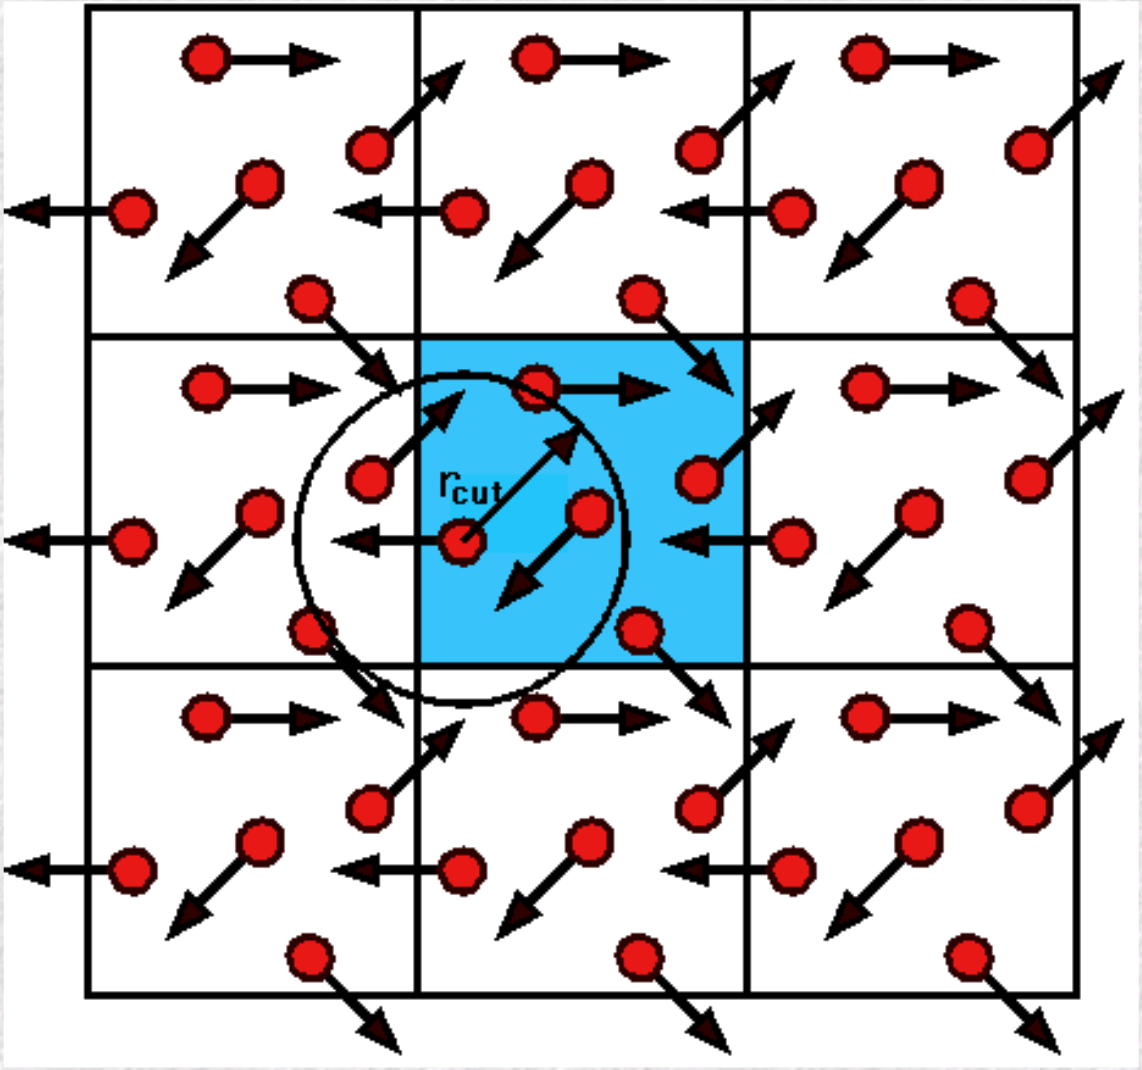
\includegraphics[width=.6\textwidth]{pbcmi1.png}
    \caption{periodic boundary condition and minimum-image convention\cite{UCLpbc}}
\end{figure}

\subsubsection{Integrating the Equations of Motion}

\begin{algorithm}[H]
    \caption{Integration of Equations of Motion}
    \begin{algorithmic}[1]
        \Function{integrate}{}
        \State sumv=0
        \State sumv2=0
        \For{i=1: npart}  \Comment{MD loop}
            \State xx=2*x(i)-xm(i)+delt**2*f(i) \Comment{Verlet algorithm}
            \State vi=(xx-xm(i))/(2*delt)   \Comment{velocity}
            \State sumv=sumv+vi    \Comment{velocity of center of mass}
            \State sumv2=sumv2+vi**2  \Comment{total kinetic energy}
            \State xm(i)=x(i)  \Comment{update previous positions}
            \State x(i)=xx   \Comment{update current positions}
        \EndFor

        \State temp=sumv2/(3*npart)  \Comment{instantaneous temperature}
        \State etot=(en+0.5*sumv2)/npart \Comment{total energy per particle}
        \State sumv=sumv/npart

        \State \textbf{return}
        \EndFunction
    \end{algorithmic}
\end{algorithm}

It is worth noting that throughout the simulation, the total energy \texttt{etot} should remain approximately constant, and the velocity of center of mass \texttt{sumv} should also remain zero.

The system we are simulating is usually non-dissipative, and we want to obtain a symplectic and reversible integrator, in order to preserve the total energy and improve robustness. Liouville theorem tells us that the Verlet or velocity Verlet algorithm satisfies these requirements. A proof can be found here \cite{ORAC}. The Verlet algorithm is characterized by the following equations
\begin{equation}
    \left\{
    \begin{aligned}
        r(t+\delta t)&=2r(t)-r(t-\delta t)+\frac{F(t)}{m}\delta t^2 \\
        v(t)&=\frac{r(t+\delta t)-r(t-\delta t)}{2\delta t}
    \end{aligned}
    \right.
\end{equation}
We only need the first equation to obtain the trajectory, but we still need the velocities to calculate the temperature and energy, thus the second equation. 

Combining the above three algorithms, we can realize a complete molecular dynamics simulation program.

\begin{algorithm}[H]
    \caption{Simple MD Program}
    \begin{algorithmic}[1]
        \State call \Call{init}{}   \Comment{initialize}
        \State t=0
        \While {t<tmax}
            \State call \Call{force}{}    \Comment{determine forces}
            \State call \Call{integrate}{} \Comment{integrate equations of motion}
            \State t=t+delt
            \State call \Call{sample}{}  \Comment{sample averages}
        \EndWhile
    \State \textbf{return}
    \end{algorithmic}
\end{algorithm}

The function \texttt{SAMPLE} is not defined in the pseudocodes above. It calculates the average quantities along the simulation trajectory.

\subsection{Monte Carlo Simulation}

As opposed to molecular dynamics, Monte Carlo simulation does not follow any real or simulated trajectories. We do not need forces or velocities. The kinetic energy or other functions that only depend on the particle velocities have averages that can be easily carried out, because the velocities follow Maxwell-Boltzmann distribution and can be averaged analytically. Therefore we only need to sample in the configuration space $\boldsymbol{r}^N$. The 3N-dimensional integral is written as 
\begin{equation}
    S=\int\limits_D{F(\boldsymbol{R})\mathrm{d}\boldsymbol{R}}
\end{equation}
where $D$ is the domain of integration. Let us assume a normalized domain $\int\limits_D{\mathrm{d}\boldsymbol{R}}=1$. Following the idea of importance sampling introduced by Metropolis, we sample $M$ random points $\boldsymbol{R}_i$ from a nonuniform probability distribution $W(\boldsymbol{R})$\cite{Comp}. Then the integral is estimated by 
\begin{equation}
    S\approx \frac{1}{M}\sum\limits_{i=1}^M\frac{F(\boldsymbol{R}_i)}{W(\boldsymbol{R}_i)}
\end{equation}
It can be shown that the standard deviation of the estimated integral from the exact integral is 
\begin{equation}
    \sigma_S^2=\left\langle\left(\frac{1}{M}\sum\limits_{i=1}^M\frac{F(\boldsymbol{R}_i)}{W(\boldsymbol{R}_i)}-\left\langle\frac{F(\boldsymbol{R})}{W(\boldsymbol{R})}\right\rangle\right)^2\right\rangle=\frac{1}{M}\left(\left\langle\frac{F^2}{W^2}\right\rangle-\left\langle\frac{F}{W}\right\rangle^2\right)
\end{equation}
To minimize $\sigma_S^2$, $G(\boldsymbol{R})=F(\boldsymbol{R})/W(\boldsymbol{R})$ should be nearly a constant. Compare this with the canonical ensemble average
\begin{equation}
    \left\langle A\right\rangle=\int\limits_{D}{A(\boldsymbol{R})W(\boldsymbol{R})\mathrm{d}\boldsymbol{R}}
\end{equation}
where the weight $W(\boldsymbol{R})$ is the probability density function
\begin{equation}
    W(\boldsymbol{R})=\frac{e^{-U(\boldsymbol{R}/k_BT)}}{\int\limits_D{e^{-U(\boldsymbol{R}'/k_BT)}\mathrm{d}\boldsymbol{R}'}}
\end{equation}
Metropolis's method generates a sequence of sample points in the configuration space. The probability of transition from the old sample point to the new sample point obeys the principle of detailed balance 
\begin{equation}
    W(\boldsymbol{R})T(\boldsymbol{R}\rightarrow\boldsymbol{R}')=W(\boldsymbol{R}')T(\boldsymbol{R}'\rightarrow\boldsymbol{R})
\end{equation}
The ratio of transition probabilities is 
\begin{equation}
    \frac{T(\boldsymbol{R}\rightarrow\boldsymbol{R}')}{T(\boldsymbol{R}'\rightarrow\boldsymbol{R})}=\frac{W(\boldsymbol{R}')}{W(\boldsymbol{R})}=e^{-(U(\boldsymbol{R}')-U(\boldsymbol{R}))/k_BT}
\end{equation}
It is easily verified that the following choice of transition probability (rate) arrives at detailed balance
\begin{equation}
    T(\boldsymbol{R}\rightarrow\boldsymbol{R}')=\min \left(1,e^{-\beta\left(U(\boldsymbol{R}')-U(\boldsymbol{R})\right)}\right)
\end{equation}
\begin{algorithm}[H]
    \caption{Metropolis algorithm}
    \begin{algorithmic}[1]
        \State call \Call{init\_position}{}  \Comment{initialize starting positions of all particles}
        \For{icycl=1: ncycl}
            \State o=randint(1, npart)  \Comment{randomly select a particle}
            \State eno=\Call{ener}{x(o)}  \Comment{old energy}
            \State xn=x(o)+randx()    \Comment{random displacement}
            \State enn=\Call{ener}{xn}  \Comment{new energy}
            \If{ranf()<exp(-beta*(enn-eno))}   \Comment{Metropolis acceptance rule}
                \State x(o)=xn
            \EndIf
            \State call \Call{sample}{}
        \EndFor
        \State \textbf{return}
    \end{algorithmic}
\end{algorithm}
Finally, a version of Metropolis Monte Carlo simulation program is established. 

\section{Simulations}
The specifications and requisites of our simulations are clearly provided in the assignment. Let us jump right into the tasks.

\subsection{TASK1}
Different potentials as functions of $r$. 
\begin{table}[H]
    \centering
    \caption{potential functions}
    \label{tab:potentials}
    
    \begin{tabular}{|c|c|c|c|}
    \hline
    \parbox[c][1.2cm][c]{2cm}{\centering Potential} & \parbox[c][0.8cm][c]{3cm}{\centering Lennard-Jones $U^{LJ}(r)$} & \parbox[c][0.8cm][c]{2.3cm}{\centering Atomic $\phi^A(r)$} & \parbox[c][0.8cm][c]{2.5cm}{\centering Colloidal $\phi^C(r)$} \\
    \hline
    \rule{0pt}{0.5cm} Minimum $r_{min}$ & $2^{1/6}$ & 1.155 & 1.055 \\
    \rule{0pt}{0.5cm} Cut-off $r_c$ & 2.5 & 2.0 & 1.2 \\
    \rule{0pt}{0.5cm}  Prefactor $\alpha$ & N.A. & 1 & 114 \\
    \hline
    \end{tabular}
    
\end{table}
Their plots are as follows.

\begin{figure}[H]
    \centering
    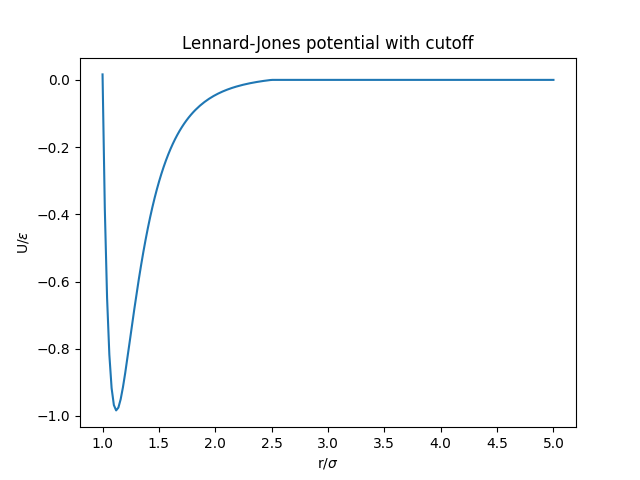
\includegraphics[width=.8\textwidth]{lj_cutoff.png}
    \caption{Lennard-Jones potential with cutoff}
\end{figure}

\begin{figure}[H]
    \centering
    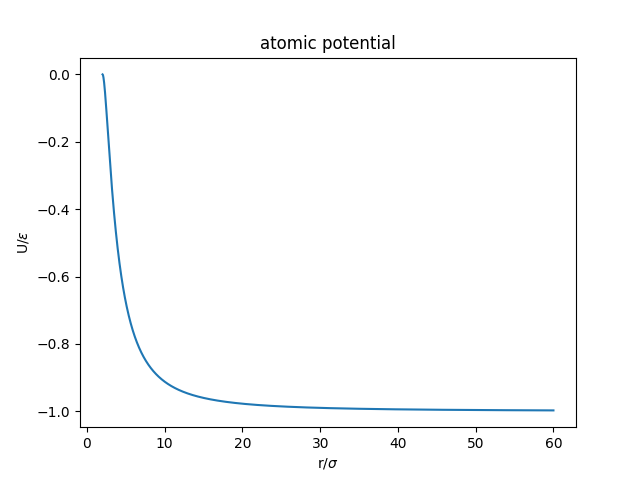
\includegraphics[width=.8\textwidth]{phi_A.png}
    \caption{atomic potential}
\end{figure}

\begin{figure}[H]
    \centering
    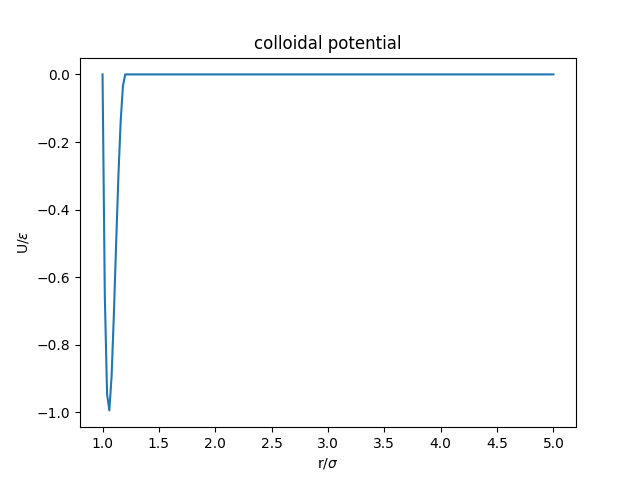
\includegraphics[width=.8\textwidth]{phi_C.png}
    \caption{colloidal potential}
\end{figure}

\subsection{TASK2}
This task requires me to do the simulation with two initial conditions: random positions and ordered lattice, using MC and MD methods. 
\subsubsection{Random positions}

\begin{enumerate}[label=(\alph*)]
    \item Monte Carlo simulation
    
    The initial configuration is generated like this 
    \begin{figure}[H]
        \centering
        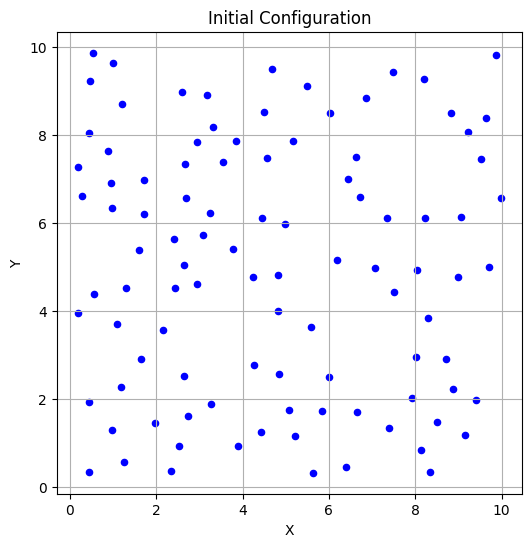
\includegraphics[width=.8\textwidth]{random_init_config.png}
        \caption{initial configuration: random positions}
    \end{figure}
    I should make sure every two particles do not overlap with each other. Using the atomic potential, and fixing the temperature and density to $T_1=0.728, \rho_1=0.8442$, I reach a final configuration like this 
    \begin{figure}[H]
        \centering
        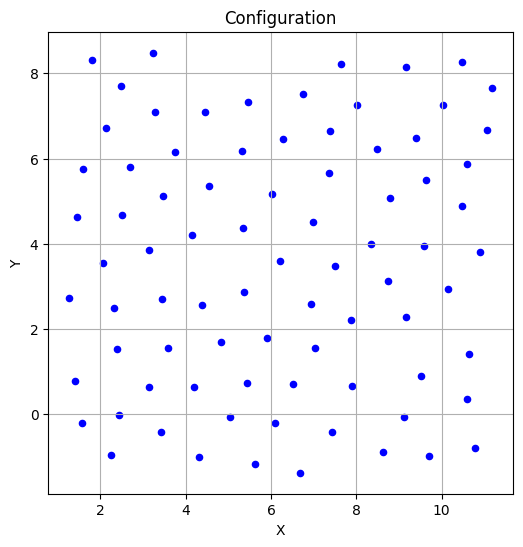
\includegraphics[width=.8\textwidth]{final_config_mc1.png}
        \caption{MC final configuration 1}
    \end{figure}
    This is after 10000 steps of simulation. The total potential energy as a function of time is plotted as follows
    \begin{figure}[H]
        \centering
        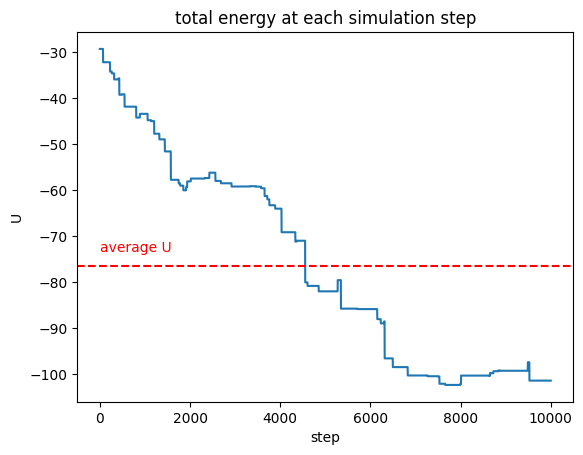
\includegraphics[width=.8\textwidth]{energy_to_time_mc1.png}
        \caption{MC energy versus step 1}
    \end{figure}
    My citerion for testing the equilibration is:
    \begin{enumerate}[label=\textbullet]
        \item The energy stays negative.
        \item The energy only fluctuates within a relatively small range, without showing a trend of increasing or decreasing.
    \end{enumerate}
    According to my criterion, the equilibrium is reached at around step 6500, so if I want to evaluate the real average energy, I can only sum up those steps after equilibrium. The result is 
    \begin{equation}
        \left \langle U\right\rangle=-100.346
    \end{equation}
    The average energy per particle is 
    \begin{equation}
        \left\langle u\right\rangle=\frac{\left \langle U\right\rangle}{N}=-1.239
    \end{equation}
    I can also analyze the fluctuation of energy
    \begin{equation}
        \delta U^2=\left \langle U^2\right\rangle-\left \langle U\right\rangle^2=1.330
    \end{equation}
    The relative fluctuation of the energy is
    \begin{equation}
        \left| \frac{\delta U}{\left \langle U\right\rangle} \right|\approx 1.15\%
    \end{equation} 

    Choosing another fixed condition $T_2=1.0,\ \rho_2=0.1$, because the density is far smaller than the previous condition, the equilibrium is sooner reached. 

    The final configuration is 
    \begin{figure}[H]
        \centering
        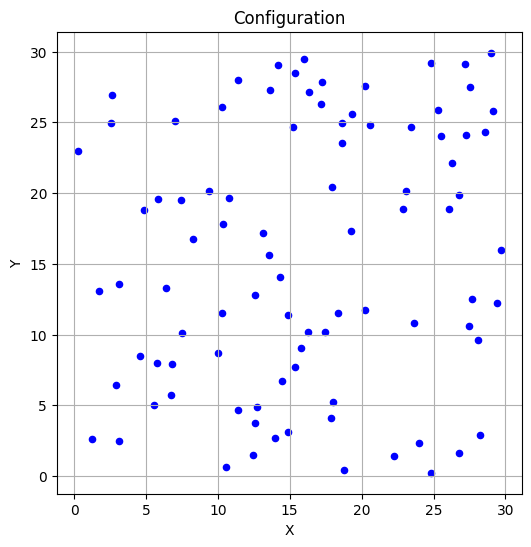
\includegraphics[width=.8\textwidth]{final_config_mc2.png}
        \caption{MC final configuration 2}
    \end{figure}
    This is after 5000 steps of simulation. The total potential energy as a function of time is plotted as follows
    \begin{figure}[H]
        \centering
        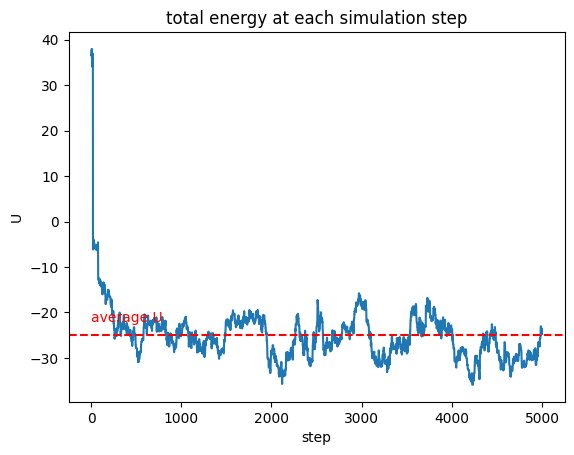
\includegraphics[width=.8\textwidth]{energy_to_time_mc2.png}
        \caption{MC energy versus step 2}
    \end{figure}
    The average energy is 
    \begin{equation}
        \left\langle U\right\rangle=-25.893
    \end{equation}
    The average energy per particle is 
    \begin{equation}
        \left\langle u\right\rangle=\frac{\left\langle U\right\rangle}{N}=-0.2877
    \end{equation}
    I can also analyze the fluctuation of energy
    \begin{equation}
        \delta U^2=\left \langle U^2\right\rangle-\left \langle U\right\rangle^2=14.90
    \end{equation}
    The relative fluctuation of the energy is
    \begin{equation}
        \left| \frac{\delta U}{\left \langle U\right\rangle} \right|\approx 14.9\%
    \end{equation}
    Obviously, higher temperature and lower density result in higher average energy and greater fluctuation in energy. 

    \item molecular dynamics simulation
    
    In MD simulation, I need to keep an eye on both the positions and velocities of the particles. In addition to solving the equations of motion, I also have to maintain a constant temperature for the $NVT$ ensemble. An Anderson thermostat is applied in my simulation. To perform the simulation with Anderson thermostat, I need two parameters: $T$ and $\nu$.  $T$ is the controlled temperature of the system, and $\nu$ is the frequency of stochastic collisions which determine the strength of the coupling to the heat bath. If successive collisions are uncorrelated, then the distribution of time intervals between two successive stochastic collisions is of Poisson form
    \begin{equation}
        P(X=k)=f(k;\lambda)=\frac{\lambda^k e^{-\lambda}}{k!}
    \end{equation}
    Its expectation value is $E(X)=\lambda$, which means after every collision, the next collision is expected to come in $\lambda$ simulation steps. The frequency of collisions is $\nu=\frac{1}{\lambda}$. 

    In a constant temperature simulation, I first specify the initial positions and momenta. Then I will integrate the equations of motion until the first stochastic collision, which happens at the time determined by a random variable following Poisson distribution. I randomly select a particle which suffers this collision, and its momentum is instantaneously switched to a value generated from Maxwell-Boltzmann distribution under temperature $T$. The Newtonian equations are then integrated until the next collision. This process is repeated to the end of the simulation.

    \vspace{\baselineskip}
    For the first set of fixed conditions, $T1=0.728,\rho_1=0.8442$, I run the simulation for 5000 steps. I have chosen $\lambda=3$, and each time step $\delta t=0.014$, getting a final configuration as the figure below 
    \begin{figure}[H]
        \centering
        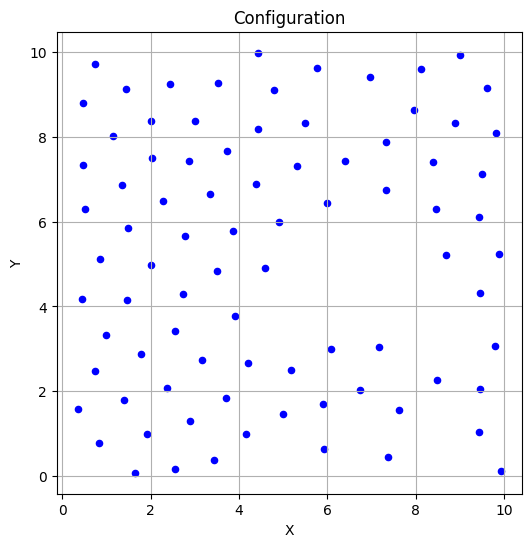
\includegraphics[width=.8\textwidth]{final_config_md1.png}
        \caption{MD final configuration 1} 
    \end{figure}
    From the final configurations of MC and MD simulations, one may be surprised to discover that the particles tend to be evenly and regularly placed in the box -- some even exhibit hexagonal or square lattice structure! But these symmetries are not presupposed. This may explain the formation of solids, especially crystals. 

    The total potential energy as a function of time is plotted as follows
    \begin{figure}[H]
        \centering
        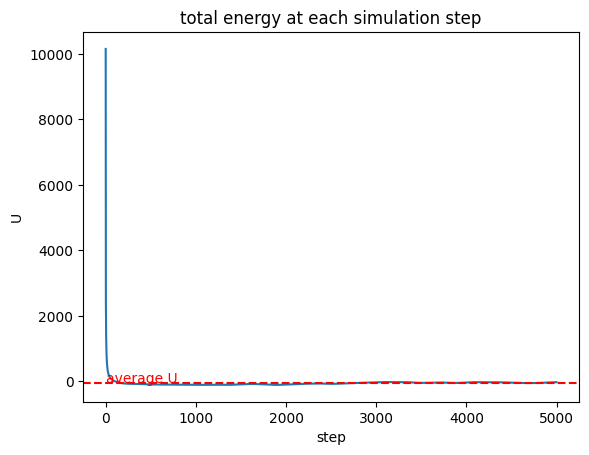
\includegraphics[width=.8\textwidth]{energy_to_time_md1.png}
        \caption{MD energy versus step 1}
    \end{figure}
    Since the initial energy is too large, I should truncate the list of energies, leaving only the equilibrium states. 
    \begin{figure}[H]
        \centering
        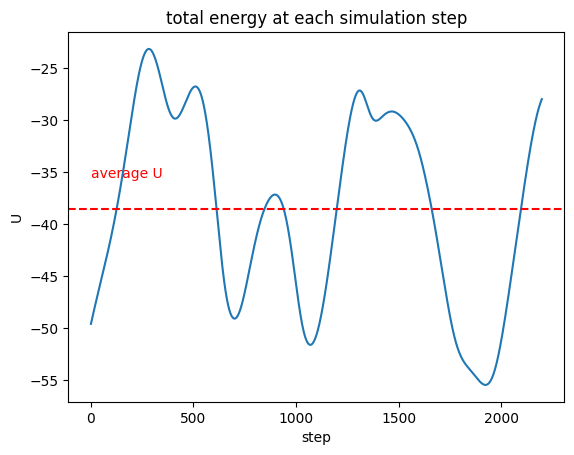
\includegraphics[width=.8\textwidth]{energy_to_time_md2.png}
        \caption{MD energy versus step 2}
    \end{figure}
    I can now calculate the statistical values 
    \begin{equation}
        \left\langle U\right\rangle=-38.557
    \end{equation}
    \begin{equation}
        \delta U^2=87.544
    \end{equation}
    It can be seen that the average energy is a lot higher than in MC simulation (for the same fixed condition), and the variance in $U$ is also larger. Although the final configuration resembles that in MC simulation, I wonder if I have not reached the real equilibrium.
    
    Therefore I reset $\lambda$ and $\delta t$, and manage to find a better equilibrium. 
\end{enumerate}

\subsubsection{Ordered lattice}

\subsection{TASK3}
The aim of this task is to study the relation between $\left\langle U\right\rangle$, $\delta U$ and the system size $N$. 

\subsection{TASK4}
This task asks me to calculate the radial distribution function $g(r)$ from the simulations. Suppose we have $N$ particles, and $\rho_N(\boldsymbol{r}_1,\cdots,\boldsymbol{r}_N)$ is called the configuration probability density, meaning that the probability for the $N$ particles being respectively in $\mathrm{d}^3\boldsymbol{r}_1,\cdots,\mathrm{d}^3\boldsymbol{r}_N$ is $\rho_N(\boldsymbol{r}_1,\cdots,\boldsymbol{r}_N)\mathrm{d}^3\boldsymbol{r}_1\cdots\mathrm{d}^3\boldsymbol{r}_N$. For a simulation box with volume $V$, the average density of the particles is $n=\frac{N}{V}$. 

We then define the pair distribution function 

\begin{equation}
    \label{Eq:pair_distri}
    F_2(\boldsymbol{r}_1,\boldsymbol{r}_2)\equiv N(N-1)\int\cdots\int\rho_N(\boldsymbol{r}_1,\cdots,\boldsymbol{r}_N)\mathrm{d}^3\boldsymbol{r}_3\cdots\mathrm{d}^3\boldsymbol{r}_N
\end{equation}

As a homogeneous system has translational invariance, $F_2(\boldsymbol{r}_1,\boldsymbol{r}_2)=F_2(\boldsymbol{r}_2-\boldsymbol{r}_1)$, we introduce the radial distribution function 
\begin{equation}
    F_2(\boldsymbol{r}_2-\boldsymbol{r}_1)\equiv n^2g(\boldsymbol{r}_2-\boldsymbol{r}_1)
\end{equation}
Integrating Eq. \ref{Eq:pair_distri}, we get

\begin{equation}
    \begin{aligned}
        N(N-1)&=\iint{F_2(\boldsymbol{r}_2-\boldsymbol{r}_1)} \\
        &=n^2\iint{g(\boldsymbol{r}_2-\boldsymbol{r}_1)\mathrm{d}\boldsymbol{r}^3}
    \end{aligned}
\end{equation}

\subsection{TASK5}

%\begin{figure}[ht] 
        % read manual to see what [ht] means and for other possible options
%        \centering \includegraphics[width=0.8\columnwidth]{sr_setup}
        % note that in above figure file name, "sr_setup",
        % the file extension is missing. LaTeX is smart enough to find
        % apropriate one (i.e. pdf, png, etc.)
        % You can add this extention yourself as it seen below
        % both notations are correct but above has more flexibility
        %\includegraphics[width=1.0\columnwidth]{sr_setup.pdf}
%        \caption{
%                \label{fig:samplesetup} % spaces are big no-no withing labels
                % things like fig: are optional in the label but it helps
                % to orient yourself when you have multiple figures,
                % equations and tables
%                Every figure MUST have a caption.
%        }
%\end{figure}

and eventually arrived to the



\section{Results and Conclusions}

Here you briefly summarize your findings. Did you learn any new physics? Was everything as expected?

In this section you will need to show your experimental results. Use tables and


In this project, TASK 2 is the most crucial part. It includes two sets of initial conditions: random positions and ordered lattice, involves two sets of fixed conditions: $T_1,\ \rho_1$ and $T_2,\ \rho_2$, and applies both the MC and MD simulation methods. To finish this task, I must have thorough understanding for both methods. Moreover, comparing results obtained from different conditions and different simulation methods, I can get a glimpse of the physics inside. 

\begin{table}[ht]
\begin{center}
\caption{Every table needs a caption.}
\label{tbl:bins} % spaces are big no-no withing labels
\begin{tabular}{|cc|} 
\hline
\multicolumn{1}{|c}{$x$ (m)} & \multicolumn{1}{c|}{$V$ (V)} \\
\hline
0.0044151 &   0.0030871 \\
0.0021633 &   0.0021343 \\
0.0003600 &   0.0018642 \\
0.0023831 &   0.0013287 \\
\hline
\end{tabular}
\end{center}
\end{table}



For example, it is easy to conclude that the
experiment and theory match each other rather well if you look at


\section{Future Work}
Since you had limited time to work on this project, what questions are left outstanding? What would be your next steps? 

%\cite{UMS}

%++++++++++++++++++++++++++++++++++++++++
% References section will be created automatically 
% with inclusion of "thebibliography" environment
% as it shown below. See text starting with line
% \begin{thebibliography}{99}
% Note: with this approach it is YOUR responsibility to put them in order
% of appearance.

\bibliography{project}


\end{document}
